\subsection*{Question 3.3}
In this question we are using this 2 equation.

\begin{equation}
	u = \frac{1}{\sqrt{\lambda_1}}k^T_1(s-\mu)
\end{equation}

\begin{equation}
	v = \frac{1}{\sqrt{\lambda_1}}k^T_1(s-\mu)
\end{equation}

Where $k_1$ and $k_2$ is the eigenvector for the to best eigenvalue. we use the original data from the hands to find there difference from this 2 hands. and plot are scatter plot over then difference, see figure \ref{fig:q33scatter}, where 0 in the x and y axes, is the best possible solution. It can also be seen that the difference hands in laying pretty close on the y axe, 

\begin{figure}[!htbp]
  \centering
  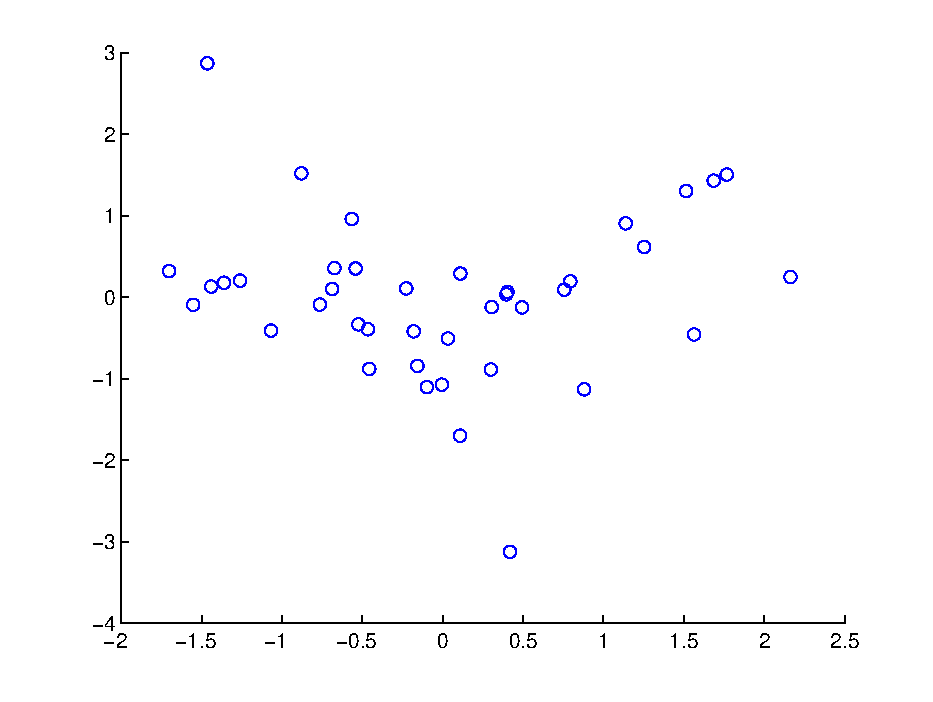
\includegraphics[width=0.85\textwidth]{./images/q33_scatter}
  \caption{Shows a scatter plot over the difference  plot over the first hand in the data set.}
  \label{fig:q33scatter}
\end{figure}

Both to point are laying long away, and sine we are calculating whit are quadratic formeler. This point where get are heigh distend. The 5 longest distends is give as $d = [10.3647, 9.9394,5.3812, 4.8844, 4.7395]$, and it is clerelig that the 2 heighest distends are ca. twice as big as the otters.
This to hands is desplete in figure \ref{fig:q33}, and it can be seen that there are big difference in them.

\begin{figure}[!htbp]
  \centering
  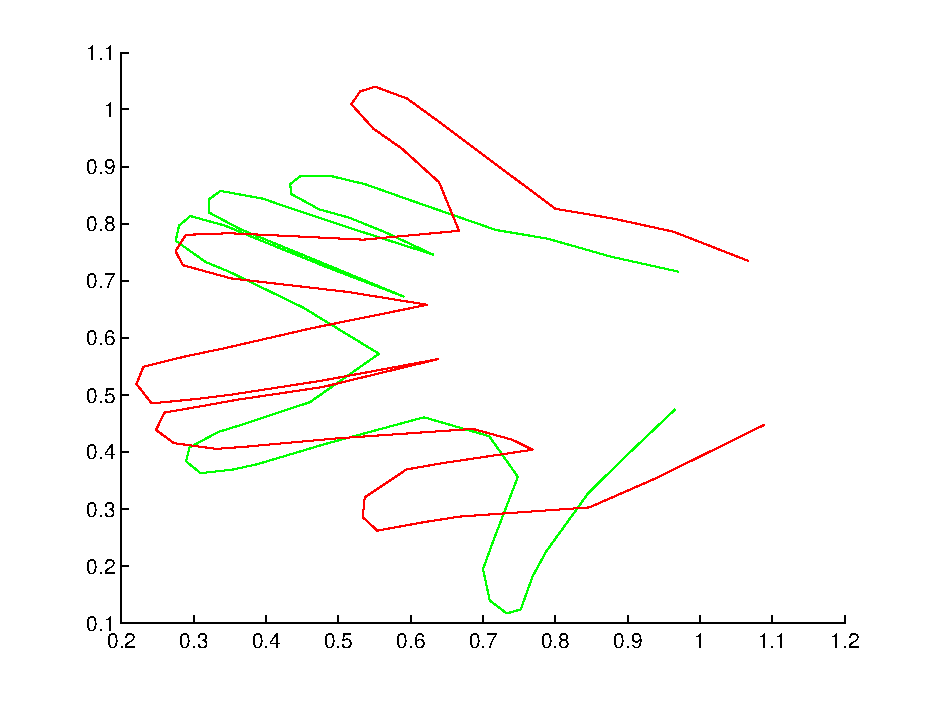
\includegraphics[width=0.85\textwidth]{./images/q33}
  \caption{To hands where the worst fit is the green hand and the scekkent worst is the red hand.}
  \label{fig:q33}
\end{figure}




